\documentclass{article}

\usepackage[paperwidth=8.5in,paperheight=11in,left=1.4in,
right=1in,top=1.3in, bottom=1.4in]{geometry}
\usepackage{sectsty, tikz, color, pgfplots}
\usetikzlibrary{shapes,arrows}
\usetikzlibrary{fit}
\makeatletter
\tikzset{
  fn/.style={
    inner sep=0pt,
    fill=none,
    draw=none,
    reset transform,
    fit={(\pgf@pathminx,\pgf@pathminy) (\pgf@pathmaxx,\pgf@pathmaxy)},
  },
  reset transform/.code={\pgftransformreset}
}
\makeatother

    \usetikzlibrary{patterns}
    \tikzset{%
        dotsfill/.style={draw,pattern=dots},
    }

\pgfdeclarepatternformonly[\StripesSize]{MyStripes}{\pgfqpoint{-1pt}{-1pt}}{\pgfqpoint{4pt}{4pt}}{\pgfqpoint{\StripesSize}{\StripesSize}}%
{
  \pgfsetlinewidth{0.3pt}
  \pgfpathmoveto{\pgfqpoint{0pt}{0pt}}
  \pgfpathlineto{\pgfqpoint{3.1pt}{3.1pt}}
  \pgfusepath{stroke}
}

\newdimen\StripesSize
\tikzset{
    StripesSize/.code={\StripesSize=#1},
    StripesSize=3pt
}

\begin{document}
\pagestyle{empty}
\begin{figure}
  \centering
    \noindent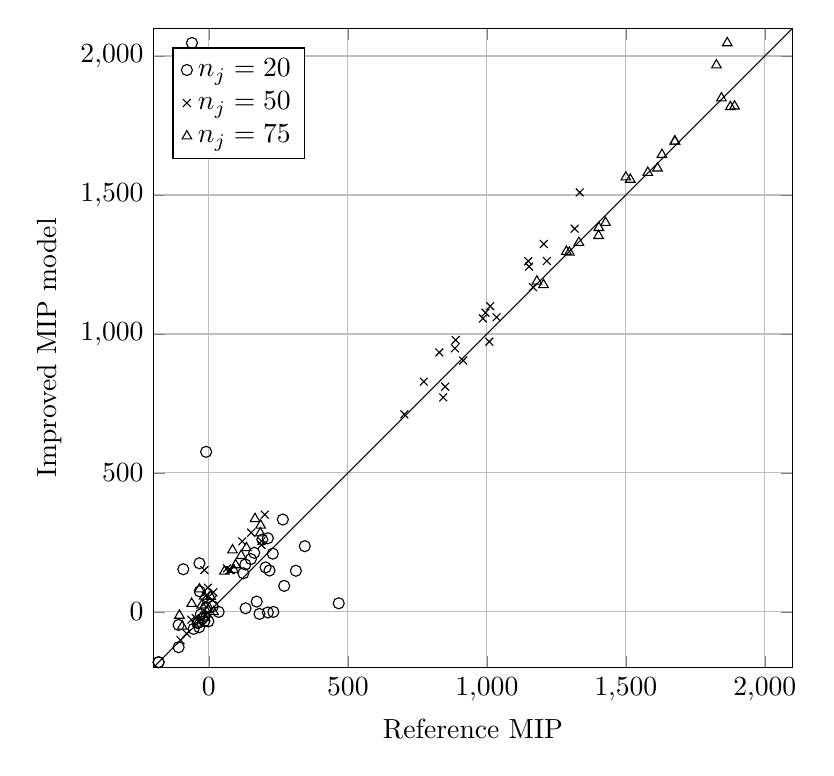
\begin{tikzpicture}

  \begin{axis}[width=0.8\textwidth, 
  height=0.8\textwidth,xmin=-200, xmax=2100, ymin=-200,
  ymax=2100,
  y tick label style={
        /pgf/number format/.cd,
            fixed,
            fixed zerofill,
            precision=0,
        /tikz/.cd
    }, 
     x tick label style={
        /pgf/number format/.cd,
            fixed,
            fixed zerofill,
            precision=0,
        /tikz/.cd
    }, grid,
    log ticks with fixed point, 
    legend pos = north west,
    xlabel=Reference MIP, ylabel=Improved MIP
    model]
\addplot[color=black, mark=o,only marks] coordinates {
(313.000053, 148)
(218.000118, 149)
(14.000085, 20)
(-180.999907, -180.999996)
(266.000073, 332.37951)
(132.000166, 13)
(-24.99989, -25)
(-60.999934, 2046.976543)
(232.000058, 0.000554)
(212.000115, 265)
(-38.99995, -39)
(-180.999841, -181)
(230.000052, 209.614731)
(124.00006, 138.946854)
(35.000115, 0)
(-39.999946, -40)
(192.000329, 260.195407)
(163.000049, 212.694861)
(-9.99986, 16.014902)
(-15.999906, -16)
(131.000279, 170.625327)
(204.00017, 160)
(-108.999855, -127)
(-109, -47)
(-9.999886, 575.928571)
(467.000066, 31)
(212.000103, -2)
(-1.999965, -34)
(-33.999839, 175.043861)
(172.000057, 37)
(271.000085, 93.688309)
(-15.999957, -33)
(-32.999902, 74)
(345.000123, 236.548617)
(182.000092, -7.063623)
(-34.999875, -55)
(-91.999933, 153.593916)
(151.000077, 190.126091)
(-54.999907, -61)
(-28.999938, -8.502134)
};
\addlegendentry{$n_j = 20$}

\addplot[color=black, mark=x,only marks] coordinates {

(1205.000326, 1323.820221)
(773.000154, 828.462892)
(16.000208, 70.368702)
(-47.37215, -22.013683)
(1316.000235, 1378.743001)
(1035.000194, 1060.152555)
(-24.999553, -24.999928)
(-79.999739, -77.823996)
(885.000168, 948.29406)
(986.000119, 1055.755943)
(120.000563, 253.843327)
(-4, -3.999941)
(843.000111, 771.720108)
(1152.000372, 1242.459579)
(-3.999639, 87.061368)
(189.001007, 240.929474)
(703.00013, 710.85604)
(888.000273, 978.194324)
(201.002333, 349.790706)
(-15.999654, 150.570364)
(1012.000226, 1099.896843)
(995.000242, 1076.54149)
(74.000283, 150.250986)
(-101.999849, -101.999992)
(1334.000289, 1509.202735)
(1216.00017, 1262.489181)
(65.000426, 156.788535)
(-11.999825, 34.189183)
(1166.00013, 1168.225321)
(915.000226, 904.470839)
(78.004276, 150.420063)
(152.000231, 285.089909)
(1009.000202, 972.263705)
(850.000368, 810.497755)
(189.001798, 254.673596)
(-62.999802, -27.937667)

(1149.000177, 1261.732246)
(829.00008, 933.650876)
(-10.999728, 57.829605)
(12.000162, 43.360814)
};
\addlegendentry{$n_j = 50$}
\addplot[color=black, mark=triangle,only marks] coordinates {
(1579.000463, 1580.562835)
(1402.000295, 1353.522649)
(17.000512, 0.000033)
(166.001395, 334.859262)
(1331.00022, 1328.778988)
(1427.000196, 1400.399817)
(-16.999763, 55.751141)
(-105.999428, -12.85891)
(1826.000142, 1967.052772)
(1286.000289, 1296.356963)
(96.000674, 168.817087)
(185.001024, 283.431971)
(1844.000242, 1848.52001)
(1614.000493, 1596.163011)
(-33.999547, 81.934169)
(-25.999464, 23.941812)
(1677.000135, 1692.93547)
(1204.00025, 1176.679462)
(-40.999467, -40.999977)
(116.002529, 202.191108)
(1876.000366, 1816.893494)
(1865.000378, 2046.976543)
(56.000721, 145.774565)
(-61.999734, 29.72713)
(1630.000472, 1645.109134)
(1403.000316, 1382.196602)
(-2.999739, 6.896751)
(135.003194, 230.39125)
(1500.000507, 1564.093624)
(1516.000473, 1555.818008)
(6.000247, 55.60861)
(-95.999577, -52.07445)
(1891.000248, 1819.305809)
(1180.00019, 1189.182575)
(85.002764, 222.414202)
(-18.999444, -18.999981)
(1676.000374, 1692.969925)
(1297.00015, 1293.732438)
(186.000237, 311.447466)
(89.00271, 152.000007)

};
\addlegendentry{$n_j=75$}


\addplot[draw=black] coordinates {(-200,-200) (2100, 2100)};

  \end{axis}
\end{tikzpicture}
   \vspace{0.73em}
\end{figure}
\end{document}
